\documentclass[12pt, oneside]{article}
\usepackage[top=1.5cm, bottom=2cm, left=2cm, right=2cm]{geometry}
\geometry{letterpaper}
\usepackage{graphicx}
\usepackage{amssymb}
\usepackage{amsmath}

\title{CPSC 530P Final Report}
\author{Neil Traft and Jolande Fooken}
\date{}

\begin{document}
\section{System and Method, or Something Like That}

\begin{itemize}
\item Describe motivation. Why classification? How is that helpful in digesting previous experience?
\item We abandoned the idea of grasp preshaping for a few reasons:
\begin{itemize}
\item The limited DOF of the Barrett Hand meant that preliminary grasp shapes would not be very interesting. Much of the end shape of a grasp is governed by the automatic TorqueSwitch\texttrademark\; mechanism in each finger [reference].
\item Our experimental setup was not suitable for the task. Realistically, it would require the objects to be fixed to the workbench. If the objects are able to move, then the hand has a tendency to push them until all three fingers are making contact. This means we would not have been able to determine separate time of contact for each finger.
\item Later in the project we had technical difficulties collecting readouts from the strain gages in the fingers. The torque measurements these provide would have been crucial in identifying the exact time of contact of each finger separately with the object. (We plan to investigate this week with Cole's help to see if there is an issue communicating with them.)
\end{itemize}
\item Experimental setup was possibly lacking. Objects' ability to move meant that the hand often settled into the same exact grasp for most objects (more or less a clamping gesture). Perhaps we should have fixed the objects to the workbench?
\end{itemize}

\subsection{Software Architecture}
The software for running our experiments on the Barrett WAM and Hand is a menu-based command-line program that makes it easy to record sensor data and test out differently trained neural networks. The menu lets the user choose between 5 different grasps:
\begin{itemize}
\item Side-on Power Grip
\item Side-on Heavy Wrap
\item Side-on Prismatic Precision
\item Top-down Prismatic Precision
\item Top-down Tripod Precision
\end{itemize}
Thus, each grasp is a combination of two factors: the position of the hand and the position of the fingers. The position of the hand, referred to as the "target position", can be either from the side (side-on) or from above (top-down). The position of fingers 1 and 2 can be at $0^\circ$ (prism), $30^\circ$ (tripod), or $180^\circ$ (wrap). When the user chooses one of the above grasps, the robot follows a fixed sequence of states:
\begin{enumerate}
\item Move to preparatory position.
\item Prepare (preshape) the hand for the particular grasp type (prism, tripod, or wrap).
\item Move to the target position (side-on or top-down).
\item Close the hand on the object.
\item Lift the object briefly and return it to the pedestal.
\item Release the object and retreat to the preparatory position.
\end{enumerate}
During steps 3-5 data is recorded from the following sensors and logged to disk:
\begin{itemize}
\item WAM joint positions
\item Finger joint positions (outer link)
\item Finger torques
\item 3D wrist forces
\item Palm and finger tactile pressures
\end{itemize}
The software is structured such that all menu options are executed asynchronously. The user always retains control and can cancel the current sequence at any time. Over time working with the robot we also found it necessary to add various facilities for identifying the name of the object currently being grasped, resetting the hand/WAM if they have controller issues, and recording a failed grasp. We use these annotations to sort and label our sensor data samples.

\textbf{Is the above section too much step-by-step? Should it be summarized?}

\begin{figure}[h]
\begin{center}
	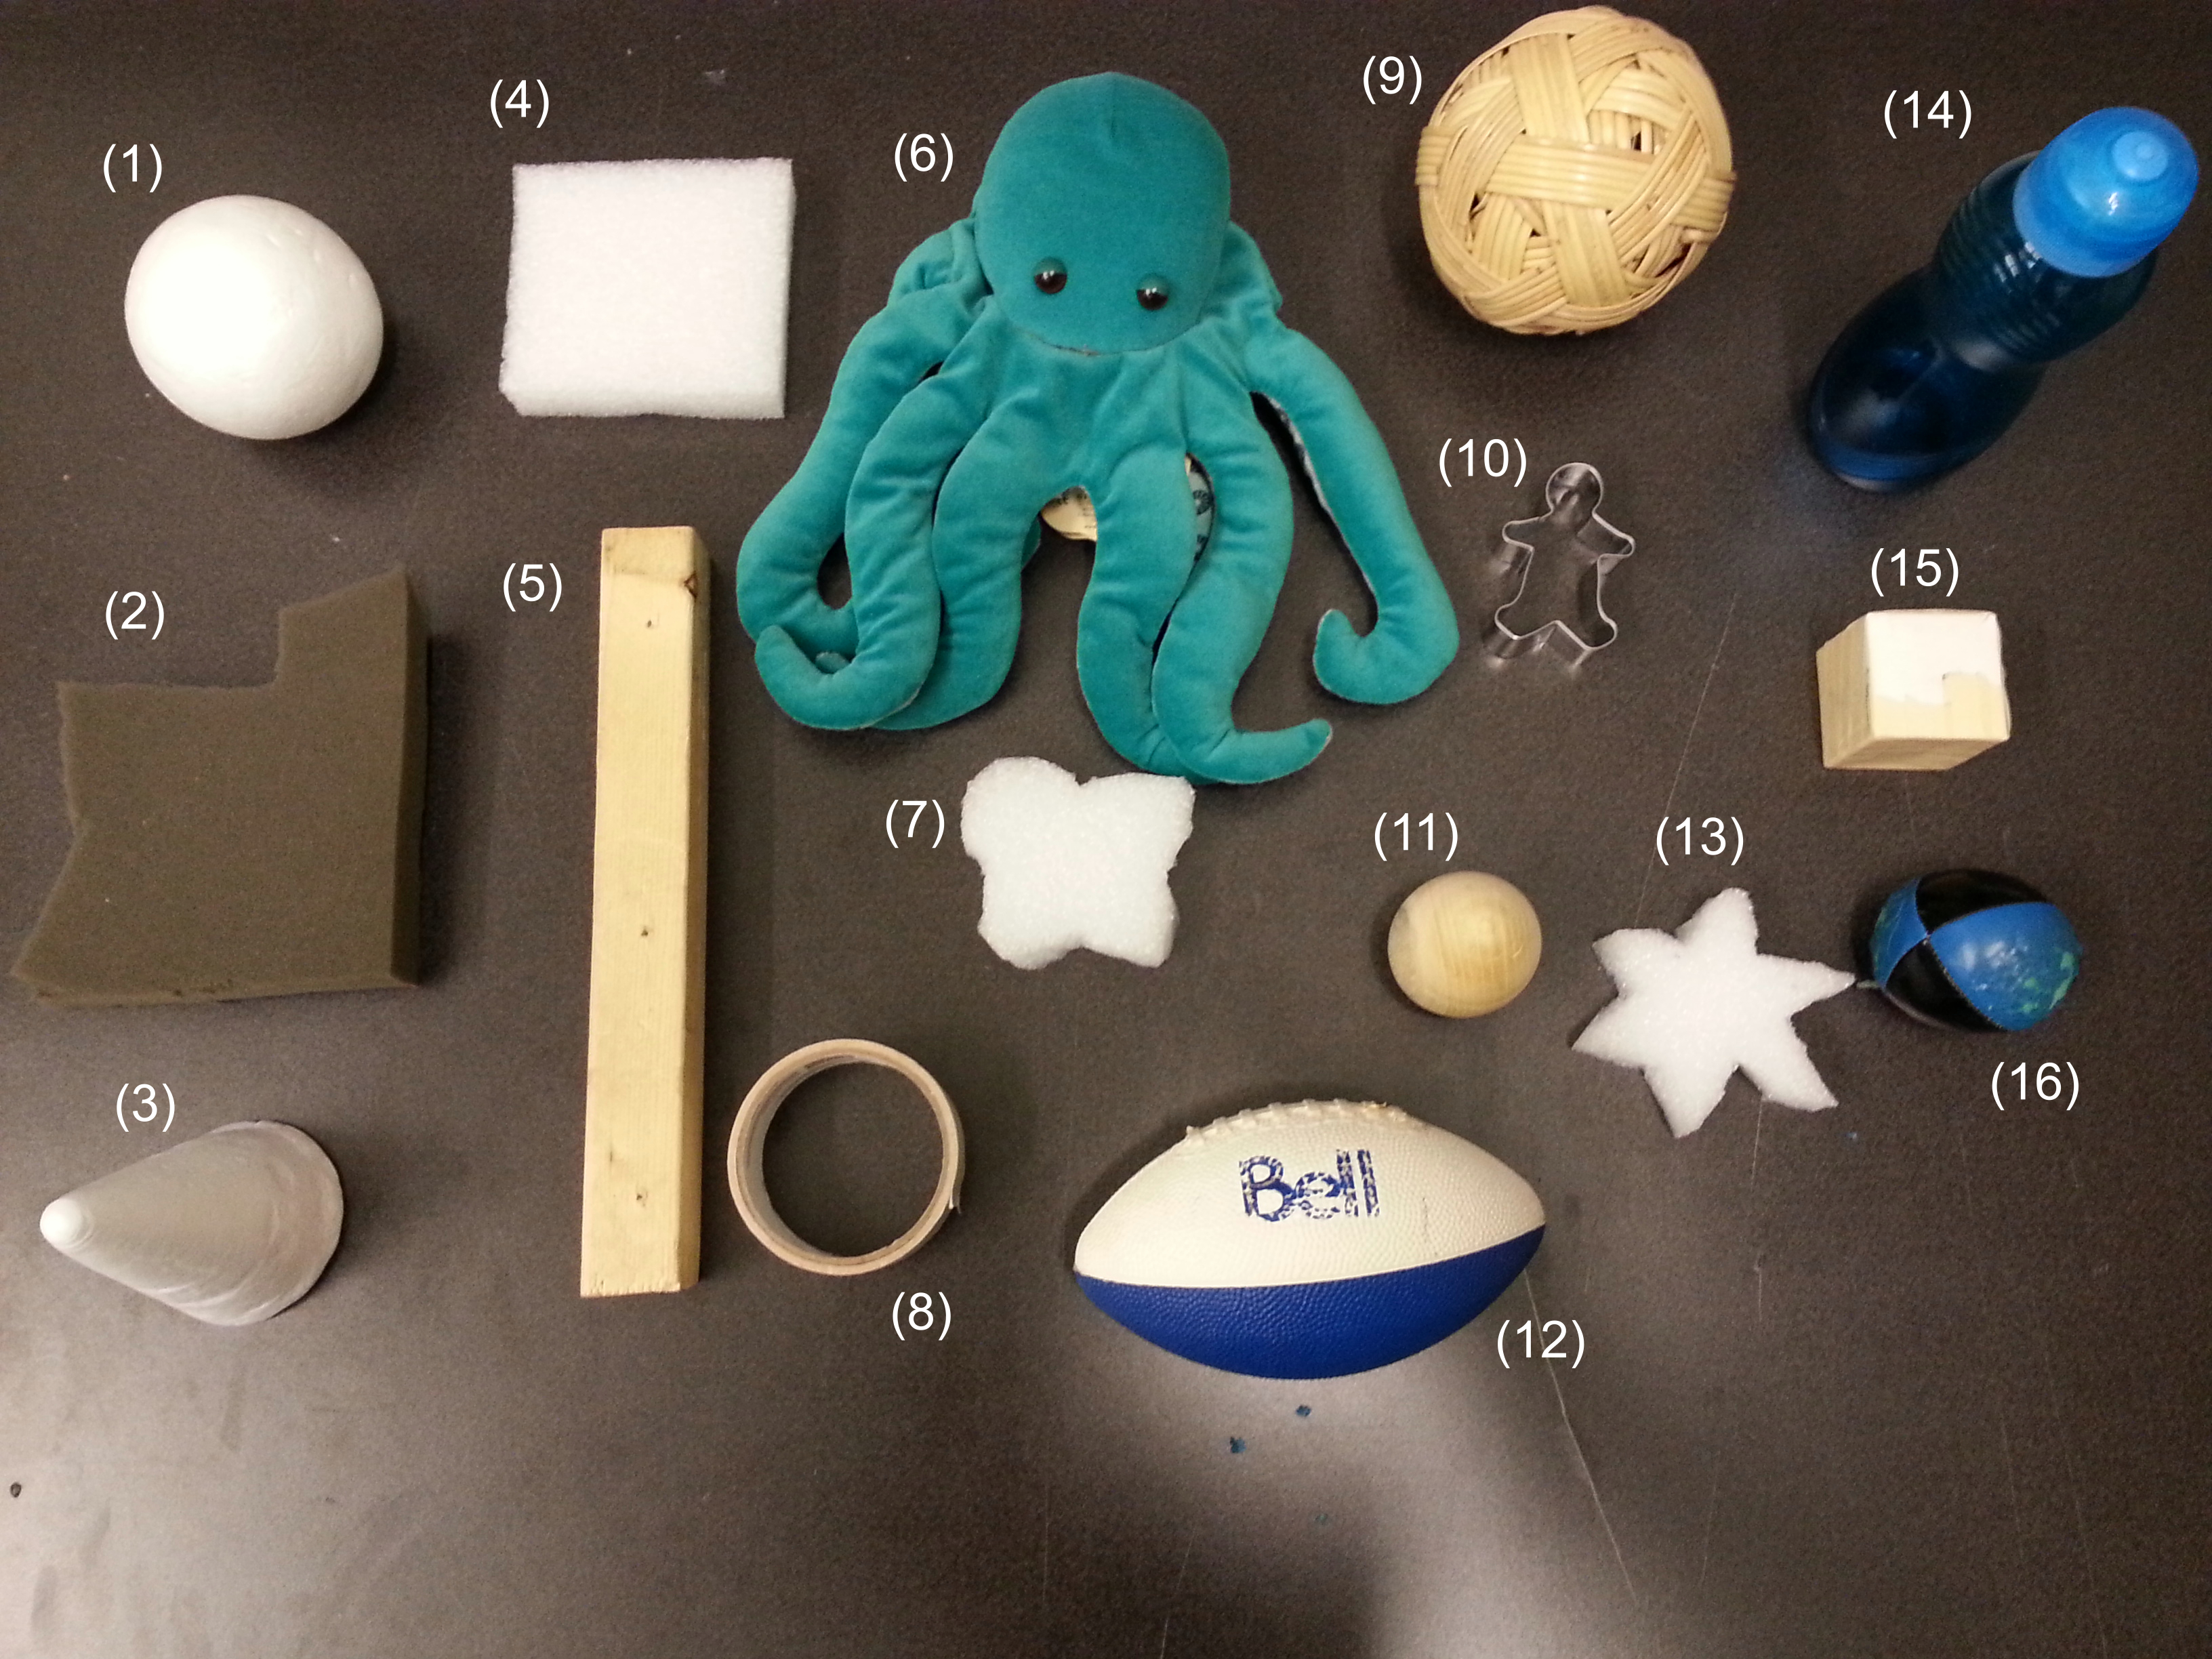
\includegraphics[width=1\textwidth]{objects.jpg}
	\caption{The set of grasped objects on which classification was performed. (1) styrofoam ball, (2) soft foam, (3) styrofoam cone, (4) foam square, (5) wood block, (6) plush octopus, (7) foam butterfly, (8) packaging tape, (9) rattan ball, (10) cookie cutter, (11) wooden egg, (12) football, (13) foam star, (14) drinking bottle, (15) cube, and (16) bean bag.}
	\label{objects}
\end{center}
\end{figure}

\subsection{The Neural Network}
To classify a grasp, the sensor data are normalized and used to train a two layer neural network. We read a total of 103 sensor values, and classify amongst 17 possible objects. Therefore the neural network consists of a 103 node input layer, a 25 node hidden layer, and a 17 node output layer. The implementation was largely borrowed from Andrew Ng's machine learning course [ref]. Since this single hidden layer with 25 nodes was enough to perform robust character recognition in [ref], it was deemed a satisfactory configuration for our purpose as well. Figure \ref{nn_config} depicts the nodes in the three layers of the neural network.

\begin{figure}[h]
\begin{center}
	\includegraphics[width=.5\textwidth]{nn.png}
	\caption{A two layer neural network for the classification of grasped objects from finger pose, wrist force, and tactile pressure data.}
	\label{nn_config}
\end{center}
\end{figure}

After the first round of experiments some neural networks were trained with the labeled data collected. We chose to focus our efforts on just 3 of the 5 grasp types, and a separate neural network was trained for each one. Each of the 103 features were separately normalized before training. 20\% of the collected time points from each grasp were set aside as a test set to verify our results. We produced a variety of different networks with different regularization weights. At this point a module was added to the software which predicted the object being grasped, given one or more samples of the above sensor data.

The final version of the software prints out the name of the object which it thinks it "feels" while lifting the object from the pedestal. It does this by taking a single time slice of sensor data while grasping an object, and feeding it forward through each layer of the neural network. The final prediction is taken as the label which was assigned the maximum probability by the output layer.

\section{Results/Conclusions}

\begin{itemize}
\item Mention that k-means clustering sorts the data very well (to what accuracy?).
\item List the changes we made to the neural network, step-by-step, to attempt to account for and eliminate the poor real-world performance: normalize data (crucial), eliminate faulty sensors, increase the regularizer, eliminate objects which may dominate feature space (can I say that? Is "dominating feature space" a thing?).
\item One way to learn from experience is to be able to \emph{classify} that experience---to place it in a category that can provide a higher level of understanding about the experience.
\item The sensor data we are collecting are compelling because they cover three different modalities. This is analogous to the mechanoreceptors of the human fingertips, which themselves cover at least three different modalities: strain, vibration, and rate of change[ref]. In our case, the modalities are mass, shape, and pliancy. The mass is given by the force/torque sensor upon lifting an object. Some parameters of the shape or at least the boundaries of the object are discribed by the finger joint positions. And finally there are the capacitive pressure sensors, which give us an estimate of the pliancy/rigidness of the object. Thus the data we collect are analogous to that of the human tactile afferents in that they are of different modalities which are orthogonal to each other, and which together create a rich description of an object for the purpose of mechanical manipulation.
\item Our hope was that raw (normalized but otherwise unprocessed) data would constitute sufficiently descriptive features to be used in classification. Our evidence shows this to be incorrect. We were unable to obtain any kind of reliable performance.
\item We are still unsure why there is such a disparity between the test set and real-world performance.
\item The fact that performance on the validation set nearly always matches performance on the training set \emph{should} indicate that no overfitting occurred. However, it may be the case that the validation data was in fact too similar to the training data: they were acquired as different time slices of the same grasp, rather than being taken from totally different grasp samples.
\item The 99\% accuracy of the neural network were suspicious and indicated that it may have overfit the data. Our tests on the robot confirmed this.
\item When run with a higher regularization weight (more regularization? heavier regularization?), the accuracy was much lower. In one example, the neural network was heavily weighted toward three or four select objects. Therefore, though overall accuracy was ~36\%, this did not indicate a good result. If run on a test set without any of these "preferred" objects, the accuracy would be near 0\%.
\item Flaws with our method even if it had worked perfectly:
\begin{itemize}
\item Limited only to objects which have been observed before.
\item Not invariant to object orientation or size. The neural network needs to have been trained with a grasp of an object in a particular orientation in order to be able to recognize that object the next time it is observed in that orientation.
\item Neither is it invariant to the shape of the hand, since we use raw sensor data rather than extracting local keypoints, as is typical in scene understanding algorithms.
\item Because of this dependence on hand and finger pose, in order to perform recognition over all the grasp types listed in Section \ref{X}, it was necessary to train a separate neural network for each type, and use the network which corresponds to the current grasp when performing predictions.
\item Likely to break down when number of objects increases. Classification gets harder the more classes you have to decide between (not to mention training gets much costlier). There is a point at which splitting hairs becomes difficult.
\end{itemize}
\item Object shapes do not necessarily show up in the pressure maps of the tactile sensor arrays. Due to the small spatial resolution of the sensor arrays, localization of shape contours is coarse. Due to the tightness of the grasps, contact surfaces with the fingers are often broad. These particular sensors probably call for a treatment very different from the edge/corner detection of computer vision algorithms.

\end{itemize}

\section{Observations/Future Work}

\begin{itemize}
\item A few specific objects dominated the network. Almost all predictions were for these objects. So it is clear what happened; what remains unclear is \emph{why} these objects dominated the neural response. Was there a feature these objects had in common that made the function reach a local mimimum there? The problem we are finding with neural networks is their opacity; it's very difficult to see inside them and understand what they are really doing.
\item If this project were continued we would produce new test sets from completely different trials with which to validate our network. The performance on this new test set, produced from a completely separate set of grasps than the training grasps, would give us more insight into the true performance of the neural network.
\item Once we finally got something working we essentially ran out of time. We would really liked to have tried some of the simple ideas we're having, now that we reflect on the experience.
\item One of the possible fixes is just to collect more samples. We collected 5-10 recordings of each grasp shape for each different object. Each grasp lasts approximately ~4 seconds and sensors are polled 20 times a second, resulting in approximately 1200-2400 samples per object. However, during the course of a single grasp, very little changes (verify this?!). Therefore, it is possible that what we have collected what amounts to only 15-30 \emph{unique} data points, which may not be enough data to train a neural network for this kind of complex recognition.
\item As illustrated by the above item, we are now painfully aware of the difficulty of collecting sufficient data for doing statistical techniques on robot experiences. Robots are often slow, and collecting recordings of their experiences in the world is time consuming and resource-intensive. One major lesson from our failure is that there may be more to gain from using what is known about human motor control, rather than unpredictable and black-box statistical techniques. Until robots are in widespread use the world over, there may not be enough variety of experiences for them to learn from by brute force alone. We should instead start from a known point using existing knowledge of human haptics and optimize from there.
\end{itemize}

\end{document}  